\section{Experiments}
\subsection{Baseline}
For our first test we need to establish a baseline to compare all other results against.  We use the \emph{even-3500} dataset using  \emph{description-unigrams} features for this baseline.  A support vector machine and a maximum entropy classifier were trained on this dataset.  The support vector machine attained 49.33\% for its testing accuracy. The testing accuracy for the maximum entropy classifier was 46.12\%.  Because there are 7 categories, random chance would put the accuracy at 14.28\%.  This means that, as a baseline, the algorithms are already performming above random chance.

\subsection{Dimensionality Reduction}
Due to the large number of features, we first attempted dimensionality reduction on the dataset as a means to increase the accuracy of the algorithm.  We attempted two dimensionlaity reductions, principle component analysis and laplacian eigenmap. Both processes were applied to the \emph{even-3500} dataset of \emph{descrption-unigrams}.  We found that the results tended to be ambiguous, in that the testing accuracy of the maximum entropy classifier tended to increase by approximately 7\% while the support vector machine had its testing accuracy decreased by 7\%.  However, except for these adjustments, the results did not change significantly.
\\

\begin{figure}[!h]
\begin{center}
\caption{Maximum Entropy with Dimensionality Reduction Testing Accuracy}
\includegraphics[width=0.7\textwidth]{Maximum_Entropy_Dimensionality_Reduction.png}
\end{center}
\end{figure}

\begin{figure}[!h]
\begin{center}
\caption{SVM with Dimensionality Reduction Testing Accuracy}
\includegraphics[width=0.7\textwidth]{SVM_Dimensionality_Reduction.png}
\end{center}
\end{figure}

Overall, it is interesting to note that there tended to be early convergence in the number of features.  Specifically, the maximum entropy classifier converged by around the 10 dimensionality mark, and the difference between 100 and 1000 for the support vector machine was significant for PCA, however, it was not significant for the laplacian eigenmap.  This seems to suggest that in natural language tasks, dimensionality reduction quickly converges to find the important features that should be used in data processing.  Though this is an interesting result, to have an accurate comparison against our baseline, further results do not include dimensionality reduction and focus instead on dataset size and feature selection.  Intuitively, because PCA tended to have a higher testing accuracy, it is suggestive that focusing on the variance of the problem was more important than attempting to keep the local proximity of the inputs constant.

\subsection{Dataset Size}
For the third set of experiments we wanted to determine to what extent more data would begin to alter the accuracy the algorithms.  We used the \emph{jagged-20000} and \emph{jagged-40000} datasets which each included \emph{description-unigrams}.

\begin{figure}[!h]
\begin{center}
\caption{Testing Accuracy with \emph{description-unigrams} features}
\begin{tabular}{| r | c | c |}
\hline
\textbf{Dataset} & \textbf{SVM} & \textbf{Maximum Entropy} \\ \hline
\emph{even-3500} & 49.33\% & 46.12\% \\ \hline
\emph{jagged-20000} & 66.87\% & 69.21\% \\ \hline
\emph{jagged-40000} & 69.53\% & 69.75\% \\ \hline
\end{tabular}
\end{center}
\end{figure}

\begin{figure}[!h]
\begin{center}
\caption{Dataset Size on Testing Accuracy}
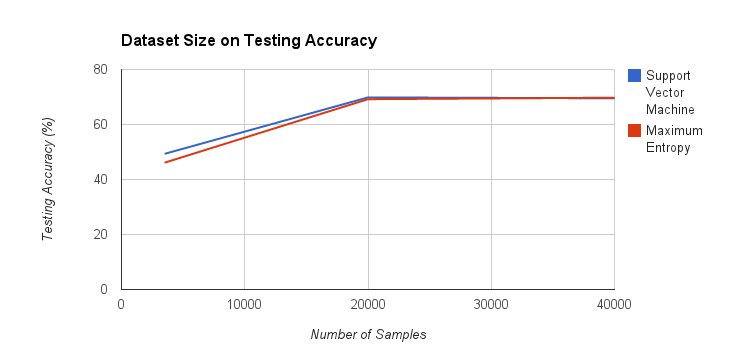
\includegraphics[width=0.7\textwidth]{Dataset_Accuracy.png}
\end{center}
\end{figure}

The size of the dataset noticeably improved the results from 3500 to 20000.  However, after this point it appears that the algorithm converged.  This is seen from the change from 20000 to 40000 samples.  The increase was nearly insignificant for the maximum entropy classifier algorithm.  To summarize, data is able to improve the testing accuracy up to a point, then gains are very small in comparison to early gains.  To further improve the results, either a different classification algorithm would need to be used, or a different set of features would need to be included.  To this end, the following set of experiments will attempt new ways of calculating the feature-vectors for each patent within the \emph{jagged-40000} dataset used in this experiment.

\subsection{Abstract-Bigrams}
For the fourth experiment, the \emph{jagged-40000} dataset was used with \emph{abstract-bigrams} used as the features.  The results indicate that the support vector machine had an accuracy of 72.12\% and the maximum entropy classifier algorithm had an accuracy of 72.57\%.  Overall, this is a slight improvement from experiment 3 of 3\% for the support vector machine and an increase of 3\% for the maximum entropy classifier.

\begin{figure}[!h]
\begin{center}
\caption{SVM with Dimensionality Reduction Testing Accuracy}
\includegraphics[width=0.7\textwidth]{Unigrams_vs_Bigrams.png}
\end{center}
\end{figure}

The small gains from this experiment were strictly due to the use of \emph{abstract-bigram} features.  This is known from the fact that only item which changed between the \emph{jagged-40000} dataset in the previous set of experiments was the move from \emph{description-unigrams} to \emph{abstract-bigrams}.  These results seem to suggest that it is still possible that further gains can be made by creating better features. Therefore, it is still of interest to attempt to create better features while using the largest possible dataset that we have.  The next experiment will attempt this experiment. 

\subsection{tf-idf}
We then used \emph{tf-idf} features on the \emph{jagged-40000} dataset.  The results showed a noticeable improvement from the original dataset, however only a slight improvement from the \emph{abstract-bigrams}.  Specifically, the score for the support vector machine was nearly identical to the \emph{abstract-bigrams}, and the maximum entropy classifier increased by ~5\% from the baseline results.

\begin{figure}[!h]
\begin{center}
\caption{tf-idf for jagged-40000 features}
\begin{tabular}{| r | c | c |}
\hline
\textbf{Features} & \textbf{SVM} & \textbf{Maximum Entropy} \\ \hline
32 & 54.37\% & 66.79\% \\ \hline
100 & 63.62\% & 71.84\% \\ \hline
250 & 72.1\% & 74.15\% \\ \hline
\end{tabular}
\end{center}
\end{figure}

\begin{figure}[!h]
\begin{center}
\caption{tf-idf Features on Testing Accuracy}
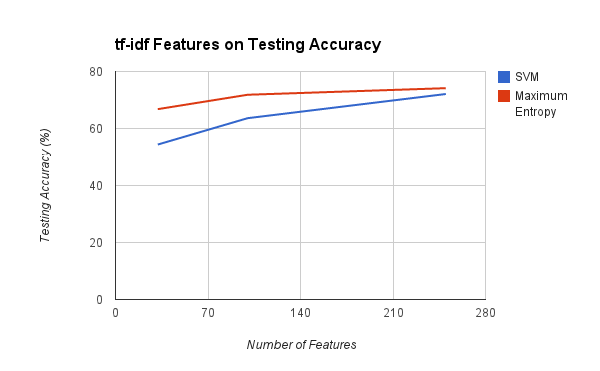
\includegraphics[width=0.7\textwidth]{tfidf.png}
\end{center}
\end{figure}

\emph{tf-idf} is a more abstract set of features that are built off of the \emph{abstract-bigrams}.  The tf-idf features only account for signification information and are therefore better at removing noise from the feature space, and the results of these features were able to further increase the accuracy of the testing algorithm for the maximum entropy classifier.  It is interesting to note, however, that the support vector machine did not gain a boost in accuracy as the maximum entropy classifier did.  Furthermore, the results gained from these features for the maximum entropy classifier were only ~2\%.  These small gains are suggestive that the new features are, in fact, able to improve the results, however the gains are beginning to decline.  It would still be interesting to attempt different features to determine if this trend holds, however, this set of abstract features did perform the best out of all other sets of features we had tested.

\subsection{Summary}

These results have a few interesting findings.  First, dimensionality reduction is able to converge quite early in terms of the dimensionality of the vectors after the process.  This is noted by the maximum entropy classifier converging early in the process, and the laplacian eigenmap for the support vector machine showing early convergence.  
\\A second finding is regarding the sample size used for the patents.  It is interesting to note that the jump from 3500 samples to 20000 samples noticeably improved the algorithm.  However, after that point, the algorithm did not gain in its testing accuracy.  This is suggestive that even when samples are doubled, results will have a tendency to converge.  This is suprising given the fact we had initially expected the results to continue to improve has more data was included.
\\Finally, the last finding of the results are regarding the abstractness of features.  \emph{description-unigrams} did the worst out of all possible sets of features in the construction of feature-vectors.  However, as the features tended to become more abstract in terms of one set of features being built off of an early set, the testing accuracy of the algorithms further improved.  This is noted by the move to \emph{abstract-bigrams} from \emph{description-unigrams} improving the testing accuracy, and furthermore the move from \emph{tf-idf} being built with \emph{abstract-bigrams} have a higher testing accuracy than only the \emph{abstract-bigrams}. Overall, we found these finding to be interesting, and a few of them even surprising.